\documentclass[12pt]{letter}
\usepackage{amsmath,amsfonts,amsthm,amstext,amssymb,graphicx, multicol,fancyhdr,lastpage,fullpage,framed,fancybox,enumerate,tikz,color,mathrsfs, polynom, tabto}
\usepackage[margin=0.6in,headsep=3pt, headheight=15pt]{geometry}

% ----------------------------------------------------------
% Custom Definitions, Commands, Environments, etc.

% Sets of numbers
\def\R{\mathbb{R}} % The reals
\def\N{\mathbb{N}} % The naturals
\def\Z{\mathbb{Z}} % The integers
\def\Q{\mathbb{Q}} % The rationals

% Blank space
\newcommand{\blank}[1]{\underline{\hspace{#1}}} % Blank space

% Change font colors
\newcommand{\cyan}[1]{{\color{cyan}{#1}}} % Changes font to cyan
\newcommand{\red}[1]{{\color{red}{#1}}} % Changes font to red
\newcommand{\magenta}[1]{{\color{magenta}{#1}}} % Changes font to magenta
\newcommand{\orange}[1]{{\color{orange}{#1}}} % Changes font to orange
\newcommand{\yellow}[1]{{\color{yellow}{#1}}} % Changes font to yellow
\newcommand{\violet}[1]{{\color{violet}{#1}}} % Changes font to violet
\newcommand{\green}[1]{{\color{green}{#1}}} % Changes font to green
\newcommand{\blue}[1]{{\color{blue}{#1}}} % Changes font to blue
\newcommand{\white}[1]{{\color{white}{#1}}} % Changes font to white

% Fitted inclusion symbols
\newcommand{\fp}[1]{\left({#1}\right)} % Fitted parentheses around content
\newcommand{\fb}[1]{\left[{#1}\right]} % Fitted brackets
\newcommand{\set}[1]{\left\{{#1}\right\}} % Fitted braces (useful for sets)
\newcommand{\av}[1]{\left|{#1}\right|} % Fitted absolute value bars

% Augmented Matrix Environment
\newenvironment{amatrix}[1]{%
	\left[\begin{array}{@{}*{#1}{c}|c@{}}
	}{%
	\end{array}\right]
}

% Miscellaneous
\def\then{\Rightarrow}
\def\to{\rightarrow}
\def\d{^{\circ}}
\newcommand{\?}{\stackrel{?}{=}}



% Coordinate Plane (Four-Quadrant)
\def\coordplane {
	\begin{tikzpicture}		\draw[step=0.25cm,black,very thin,opacity=0.25] (-2.5cm, -2.5cm) grid (2.5cm, 2.5cm);
	\draw[<->,thick,black] (-2.5cm, 0) -- (2.5cm, 0) node[anchor=north west,pos=0.94,font=\scriptsize]{$x$};
	\draw[<->,thick,black] (0,-2.5cm) -- (0, 2.5cm) node[anchor=south east,font=\scriptsize,pos=0.94]{$y$};
	\end{tikzpicture}
}

% Coordinate Plane (One-Quadrant)
\def\onequad {
	\begin{tikzpicture}
	\draw[step=0.25cm, black, very thin, opacity=0.25] (0,0) grid (7.5cm,5cm);
	\draw[->, thick, black] (0,0) -- (7.5cm, 0) node[anchor=north west,font=\scriptsize,pos=0.94]{$x$};
	\draw[->, black, thick] (0,0) -- (0,5cm) node[anchor=south east,font=\scriptsize,pos=0.94]{$y$};
	\end{tikzpicture}
}

% Counters
\newcounter{exercise}

% Exercise environment (auto-numbered)
\newenvironment{exercise}[1][]{\begin{framed}\refstepcounter{exercise}\textbf{Exercise~\theexercise:} #1}{\end{framed}}

% Book exercise environment
\newenvironment{bex}[2][] {
	\begin{framed}
		\textbf{Book Exercise {#2}}#1
	\end{framed}
}
% ----------------------------------------------------------

% ----------------------------------------------------------
% Header and Footer Information
% \pagestyle{fancy}
% \fancyhf{}
% \renewcommand{\headrulewidth}{0pt}
% \rhead{Name: \blank{2in}}
% \lhead{@}
% \rfoot{Page \thepage \, of \,\pageref{LastPage}}
% ----------------------------------------------------------
\author{Jacob Ayers}

\begin{document}
	\textbf{Assignment 6 Key \\ MAT 130}
	
	\begin{bex}{3.1.5}
		{
			
		}
	\end{bex} \vspace{-8pt}
	
	% My answer here
	The function represents a shift down of two units. The correct answer is (b).
	
	% \vspace{}
	\vfill % \newpage
	
	\begin{bex}{3.1.6}
		{
			
		}
	\end{bex} \vspace{-8pt}
	
	% My answer here
	The function represents a shift left of one unit, and a shift down of two units. The correct answer is (a).
	
	% \vspace{}
	\vfill % \newpage
	
	\begin{bex}{3.1.7}
		{
			
		}
	\end{bex} \vspace{-8pt}
	
	% My answer here
	The function represents a reflection across the $x$-axis, and a shift right of four units. The correct answer is (c).
	
	% \vspace{}
	\vfill % \newpage
	
	\begin{bex}{3.1.8}
		{
			
		}
	\end{bex} \vspace{-8pt}
	
	% My answer here
	The function represents a reflection across the $x$-axis, a shift right of two units, and a shift up of four units. The answer is (d).
	
	% \vspace{}
	\vfill % \newpage
	
	\begin{bex}{3.1.48}
		{
			
		}
	\end{bex} \vspace{-8pt}
	
	% My answer here
	The graph shows $x$-intercepts at $(-1, 0)$ and at $(5, 0)$. \begin{flalign*}
	x^2 - 4x - 5 &= 0 & \\
	(x - 5)(x + 1) &= 0 & \\
	x &= \set{-1, 5}
	\end{flalign*}
	
	% \vspace{}
	\vfill \newpage
	
	\begin{bex}{3.1.66}
		{
			
		}
	\end{bex} \vspace{-8pt}
	
	% My answer here
	Let $x$ represent the first positive real number \\
	$y$ = the second positive real number
	
	The problem statement gives the following equation: $x + 3y = 42$. Solving for $x$, we have that $x = 42 - 3y$.
	
	Our objective is to maximize the product of $x$ and $y$, $xy$. \begin{flalign*}
	xy &= (42 - 3y)y & \\
	&= -3y^2 + 42y
	\end{flalign*}
	Since $a < 0$, we know that this expression has a maximum value when $y = -\dfrac{b}{2a}$. \begin{flalign*}
	-\dfrac{b}{2a} &= -\dfrac{42}{2(-3)} & \\
	&= \dfrac{-42}{-6} & \\
	&= 7
	\end{flalign*}
	So the values of $x$ and $y$ that maximize the product $xy$ are $y = 7$ and $x = 42 - 3(7) = 21$.
	
	% \vspace{}
	\vfill % \newpage
	
	\begin{bex}{3.1.68}
		{
			
		}
	\end{bex} \vspace{-8pt}
	
	% My answer here
	(a) When the ball is punted, its horizontal distance is $0$. So we need to evaluate $f(0)$. The height of the ball when it is punted is $1.5$ ft.
	
	(b) To find the maximum height, we must evaluate $f\fp{-\dfrac{b}{2a}}$. \begin{flalign*}
	-\dfrac{b}{2a} &= -\dfrac{\frac95}{2\fp{-\frac{16}{2025}}} & \\
	&= \dfrac{-\frac95}{-\frac{32}{2025}} & \\
	&= \dfrac{9}{5} \cdot \dfrac{2025}{32} & \\
	&= 9\cdot \dfrac{405}{32} & \\
	&= \dfrac{3645}{32} & \\
	f\fp{\dfrac{3645}{32}} &= -\dfrac{16}{2025}\fp{\dfrac{3645}{32}}^2 + \dfrac95\fp{\dfrac{3645}{32}} + 1.5 & \\
	&= -102.515625 + 205.03125 + 1.5 & \\
	&\approx 104.02 \text{ ft}
	\end{flalign*} \vfill \newpage
	(c) The punt ends when it hits the ground. We are being asked to determine the value of $x$ for which $f(x) = 0$. \begin{flalign*}
	-\dfrac{16}{2025}x^2 + \dfrac95 x + 1.5 &= 0 & \\
	-16x^2 + 3645x + 3037.5 &= 0 & \\
	x &= \dfrac{-3645 \pm \sqrt{3645^2 - 4(-16)(3037.5)}}{2(-16)} & \\
	&= \dfrac{-3645\pm\sqrt{13480425}}{-32} & \\
	&\approx \dfrac{-3645\pm 3671.569828}{-32} & \\
	&\approx \dfrac{-3645 + 3671.569828}{-32} \approx -0.83 & \\
	&\approx \dfrac{-3645-3671.569828}{-32} \approx 228.64
	\end{flalign*}
	The negative answer doesn't make sense; the ball traveled about $228.64$ feet (about 76 yards).
	
	% \vspace{}
	\vfill % \newpage
	
	\begin{bex}{3.1.70}
		{
			
		}
	\end{bex} \vspace{-8pt}
	
	% My answer here
	First, rewrite the equation in the form $f(x) = ax^2 + bx + c$: $f(x) = -0.5x^2 + 20x + 230$.
	
	We are asked to find the expenditure on advertising (value of $x$) that will maximize profit. We know that $x = -\dfrac{b}{2a}$. \begin{flalign*}
	-\dfrac{b}{2a} &= -\dfrac{20}{2(-0.5)} & \\
	&= \dfrac{-20}{-1} & \\
	&= 20
	\end{flalign*}
	The expenditure on advertising that yields a maximum profit is \$2000 (since $x$ is measured in hundreds of dollars).
	
	% \vspace{}
	\vfill % \newpage
	
	\begin{bex}{3.1.72}
		{
			
		}
	\end{bex} \vspace{-8pt}
	
	% My answer here
	(a) $R(4) = -12(4)^2 + 150(4) = \$408$ \\
	$R(6) = -12(6)^2 + 150(6) = \$468$ \\
	$R(8) = -12(8)^2 + 150(8) = \$432$
	
	\vfill \newpage
	
	(b) To find the price that maximizes revenue, we need to evaluate $-\dfrac{b}{2a}$. We can then substitute that value of $p$ into the revenue function to find the maximum revenue. \begin{flalign*}
	-\dfrac{b}{2a} &= -\dfrac{150}{2(-12)} & \\
	&= \dfrac{-150}{-24} & \\
	&= \$6.25 & \\
	f(6.25) &= -12(6.25)^2 + 150(6.25) & \\
	&= \$468.75
	\end{flalign*}
	The maximum revenue is \$468.75, and it occurs when the price is \$6.25 per pet.
	
	% \vspace{}
	\vfill % \newpage
	
	\begin{bex}{3.2.20}
		{
			
		}
	\end{bex} \vspace{-8pt}
	
	% My answer here
	The degree is $2$ (even) and the leading coefficient is $2$ (positive). So the end behavior is:
	
	As $x \to -\infty$, $f(x) \to \infty$ \\
	As $x \to \infty$, $f(x) \to \infty$
	
	% \vspace{}
	\vfill % \newpage
	
	\begin{bex}{3.2.26}
		{
			
		}
	\end{bex} \vspace{-8pt}
	
	% My answer here
	First, write in polynomial form: $h(x) = -0.5x^5 - 2.7x^3 + 1$. The degree is $5$ (odd) and the leading coefficient is $-0.5$ (negative). So the end behavior is:
	
	As $x \to -\infty$, $f(x) \to \infty$ \\
	As $x \to \infty$, $f(x) \to -\infty$
	
	% \vspace{}
	\vfill % \newpage
	
	\begin{bex}{3.2.28}
		{
			
		}
	\end{bex} \vspace{-8pt}
	
	% My answer here
	First, write in polynomial form: $h(t) = -\dfrac43\fp{2t^4 - 6t^3 + t + 9} = -\dfrac83 t^4 + 8t^3 - \dfrac43 t - 12$. The degree is $4$ (even) and the leading coefficient is $-\dfrac83$ (negative). So the end behavior is:
	
	As $x \to -\infty$, $f(x) \to -\infty$ \\
	As $x \to \infty$, $f(x) \to -\infty$
	
	% \vspace{}
	\vfill % \newpage
	
	\begin{bex}{3.2.42}
		{
			
		}
	\end{bex} \vspace{-32pt}
	
	% My answer here
	\begin{flalign*}
	x^4 - x^3 - 30x^2 &= 0 & \\
	x^2\fp{x^2 - x - 30} &= 0 & \\
	x^2(x - 6)(x + 5) &= 0
	\end{flalign*}
	(a) and (b): The function has zeros at $x = 0$ (even multiplicity), $x = 6$ (odd multiplicity), and $x = -5$ (odd multiplicity).
	
	(c) The maximum possible number of turning points is $4 - 1 = 3$. \vfill \newpage
	
	(d) 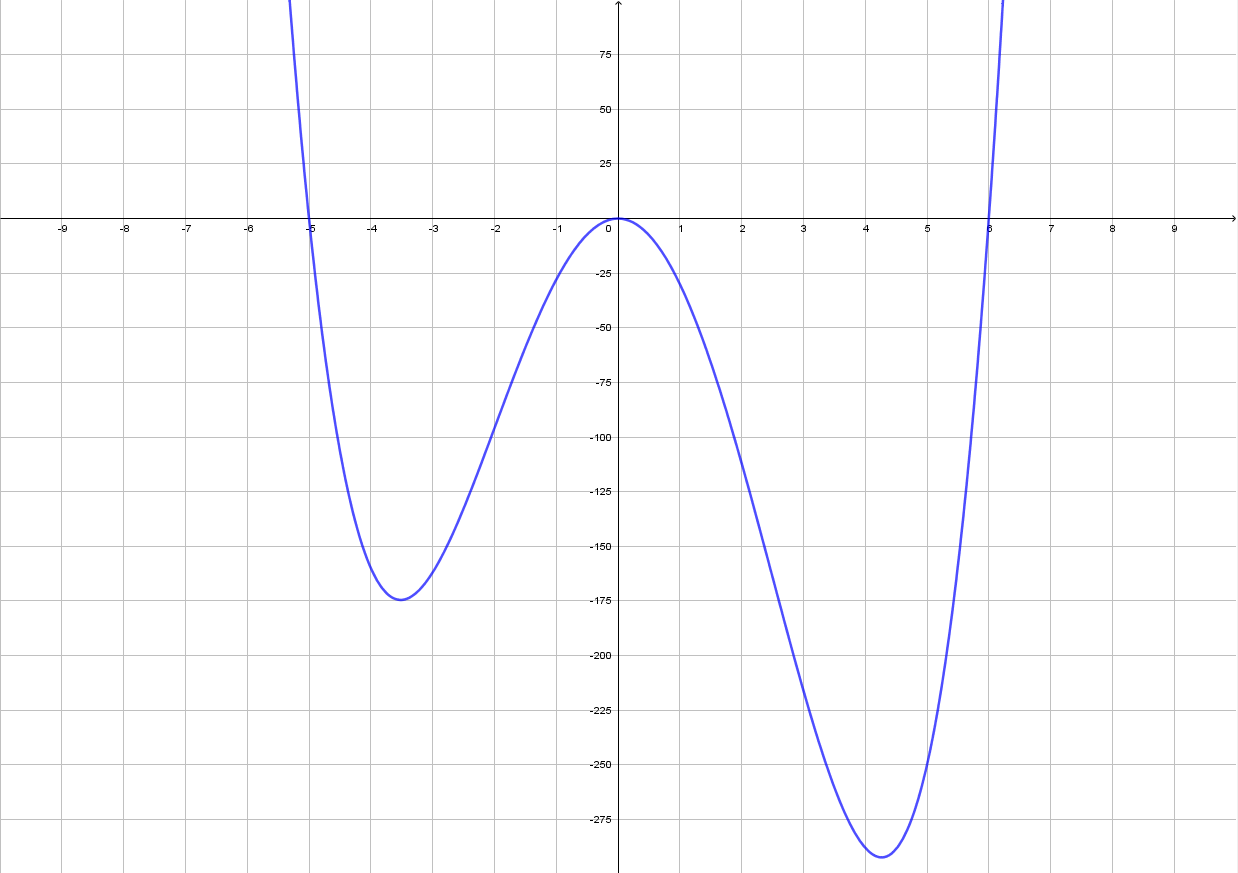
\includegraphics[width=3in]{3242d.png} \\
	The fact that the graph crosses the $x$-axis at $x = -5$ and at $x = 6$ confirms that these zeros have odd multiplicity, while the fact that the graph touches the $x$-axis at $x = 0$ confirms that this zero has even multiplicity. There are indeed 3 turning points as well.
	
	% \vspace{}
	\vfill % \newpage
	
	\begin{bex}{3.2.44}
		{
			
		}
	\end{bex} \vspace{-32pt}
	
	% My answer here
	\begin{flalign*}
	x^5 + 3^3 - 6x &= 0 & \\
	x\fp{x^4 + x^2 - 6} &= 0 & \\
	\text{Let }u &= x^2 & \\
	x\fp{u^2 + u - 6} &= 0 & \\
	x(u + 3)(u - 2) &= 0 & \\
	x\fp{x^2 + 3}\fp{x^2 - 2} &= 0 & \\
	x &= \set{\pm i\sqrt{3}, 0, \pm\sqrt{2}}
	\end{flalign*}
	(a) and (b): The function has zeros at $x = \pm i\sqrt{3}$, $x = 0$, and $x = \pm\sqrt{2}$ (a total of five zeros, all of odd multiplicity).
	
	(c) There are a maximum of $5 - 1 = 4$ turning points, but since two of the zeros are imaginary, there will be fewer than four.
	
	(d) 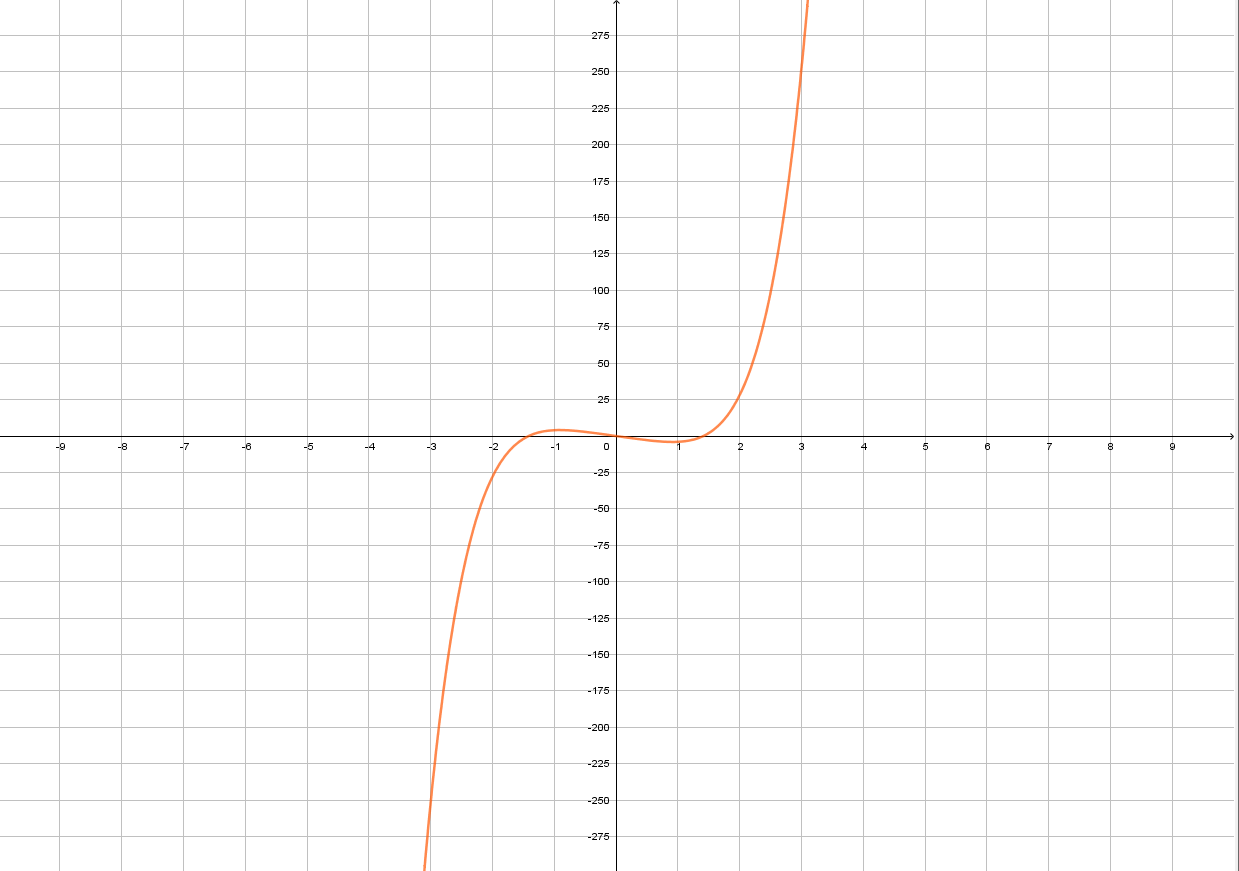
\includegraphics[width=3in]{3244d.png} \\
	We can see that the graph crosses that $x$-axis at all three real zeros, confirming that they are of odd multiplicity. There are only two turning points, but this does not violate our statement that there are a \textit{maximum} of four.
	
	% \vspace{}
	\vfill \newpage
	
	\begin{bex}{3.2.74}
		{
			
		}
	\end{bex} \vspace{-8pt}
	
	% My answer here
	(a) First, write in polynomial form: $g(x) = x^4 - 9x^2$. Now, the degree is $4$ (even) and the leading coefficient is $1$ (positive). So the end behavior is:
	
	As $x \to -\infty$, $f(x) \to \infty$ \\
	As $x \to \infty$, $f(x) \to \infty$
	
	(b) \begin{flalign*}
	x^4 - 9x^2 &= 0 & \\
	x^2\fp{x^2 - 9} &= 0 & \\
	x^2(x + 3)(x - 3) &= 0
	\end{flalign*}
	So $g$ has zeros at $x = 0$ (even multiplicity) and at $x = \pm 3$ (both odd multiplicity). It will cross the $x$-axis at $(-3, 0)$ and at $(3, 0)$, and it will touch the $x$-axis at $(0, 0)$
	
	(c) We know what the value of $g(x)$ is at the following values of $x$: $-3, 0, 3$. In order to get a more accurate sketch, it would be helpful to know the value of $g(x)$ at the following values of $x$: $-4, -2, -1, 1, 2, 4$. I used the table feature of a graphing calculator to obtain the following values:
	
	\begin{tabular}{c|cccccc}
		$x$ & $-4$ & $-2$ & $-1$ & $1$ & $2$ & $4$ \\ \hline
		$g(x)$ & $112$ & $-20$ & $-8$ & $-8$ & $-20$ & $112$
	\end{tabular}

	(d) With the information we gathered in the previous parts of the exercise, we can make an accurate sketch of the function. I used a scale of 1 block = 1 unit for the $x$-axis and 1 block = 5 units for the $y$-axis. \\
	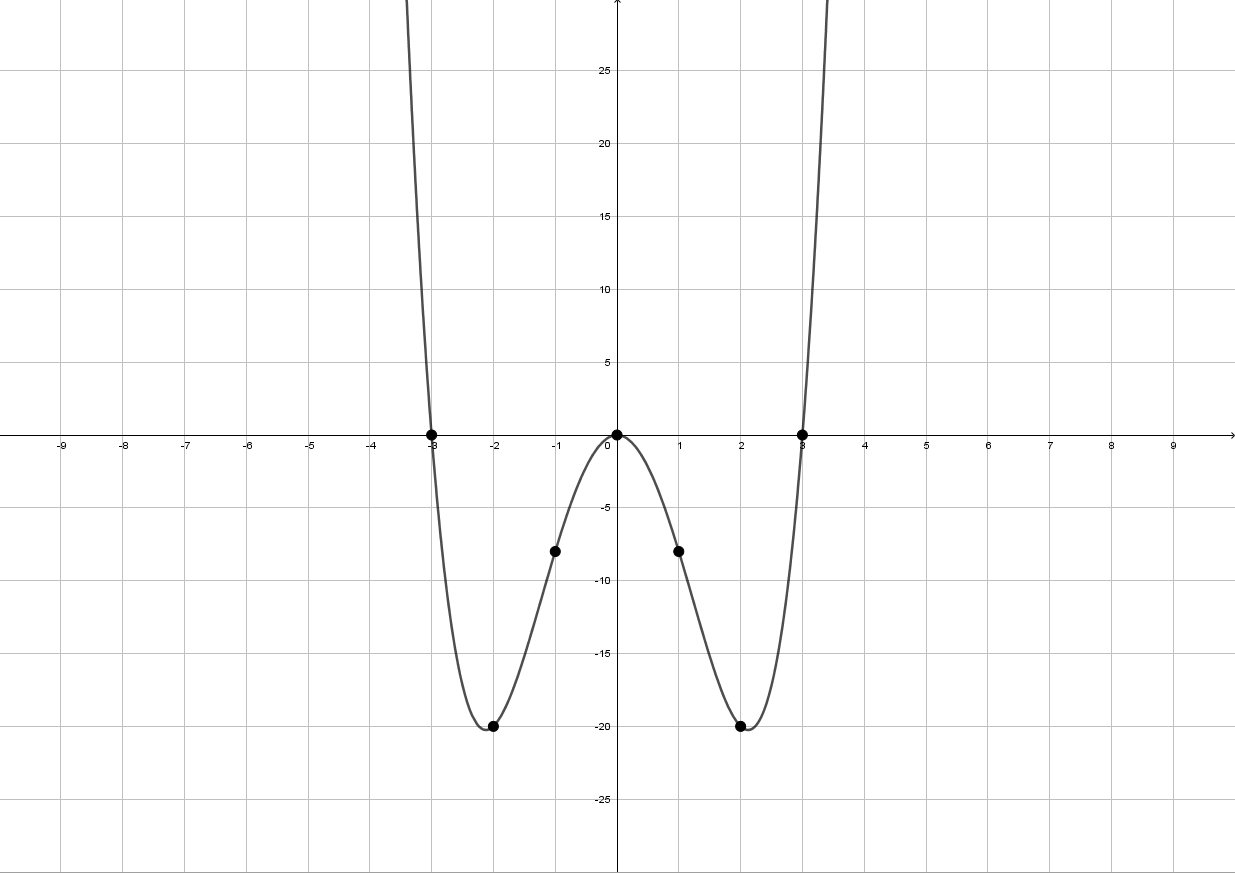
\includegraphics[width=3in]{3274d.png}
	
	% \vspace{}
	\vfill \newpage
	
	\begin{bex}{3.2.78}
		{
			
		}
	\end{bex} \vspace{-8pt}
	
	% My answer here
	(a) The degree is $3$ (odd) and the leading coefficient is $-4$ (negative). So the end behavior is:
	
	As $x \to -\infty$, $f(x) \to \infty$ \\
	As $x \to \infty$, $f(x) \to -\infty$
	
	(b) \begin{flalign*}
	-4x^3 + 4x^2 + 15x &= 0 & \\
	-x\fp{4x^2 - 4x - 15} &= 0 & \\
	-x\fp{4x^2 + 6x - 10x - 15} &= 0 & \\
	-x\fb{2x(2x+3) - 5(2x + 3)} &= 0 & \\
	-x\fp{2x - 5}\fp{2x+3} &= 0
	\end{flalign*}
	So $f$ has zeros as $x = 0$, $x = -\dfrac32$, and $x = \dfrac52$ (all odd multiplicity). The graph of $f$ will cross the $x$-axis at each of these values.
	
	(c) We know the value of $f(x)$ at the following values of $x$: $-1.5, 0, 2.5$. Here are some additional points that will aid in making our sketch (used table feature of a graphing calculator):
	
	\begin{tabular}{c|cccccccc}
		$x$ & $-4$ & $-3$ & $-2$ & $-1$ & $1$ & $2$ & $3$ & $4$ \\ \hline
		$f(x)$ & $260$ & $99$ & $18$ & $-7$ & $15$ & $14$ & $-27$ & $-132$
	\end{tabular}

	(d) With the information we gathered in the previous parts of the exercise, we can make an accurate sketch of the function. I used a scale of 1 block = 1 unit for the $x$-axis and 1 block = 5 units for the $y$-axis. \\
	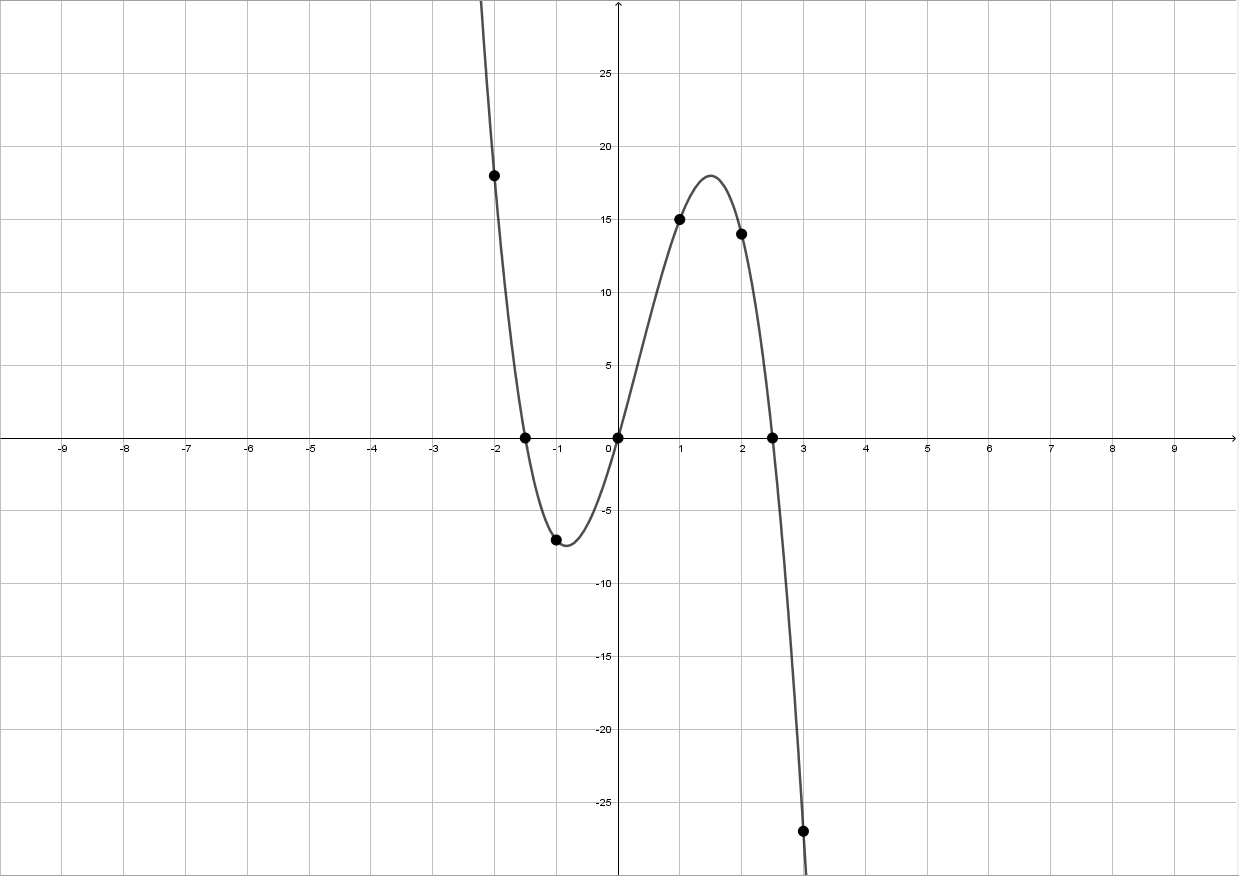
\includegraphics[width=3in]{3278d.png}
	
	% \vspace{}
	\vfill \newpage
	
	\begin{bex}{3.2.90}
		{
			
		}
	\end{bex} \vspace{-8pt}
	
	% My answer here
	(a) Using the table feature of a graphing calculator, I determined the following: \\
	$f(0) = -6.88$ and $f(1) = 0.97$, so there is a zero in the interval $(0, 1)$ \\
	$f(6) = 1.22$ and $f(7) = -1.91$, so there is a zero in the interval $(6, 7)$ \\
	$f(11) = -3.03$ and $f(12) = 2.84$, so there is a zero in the interval $(11, 12)$
	
	(b) Continuing this process, I found that there will be a zero in each of the following intervals: $(0.845, 0.846)$, $(6.385, 6.386)$, $(11.587, 11.589)$
	
	% \vspace{}
	\vfill % \newpage
	
	\begin{bex}{3.3.16}
		{
			
		}
	\end{bex} \vspace{-8pt}
	
	% My answer here
	$\polylongdiv{x^3 + 4x^2 - 3x - 12}{x - 3}$
	
	So $\fp{x^3 + 4x^2 - 3x -12} \div \fp{x - 3} = x^2 + 7x + 18 + \dfrac{42}{x-3}$
	
	% \vspace{}
	\vfill % \newpage
	
	\begin{bex}{3.3.22}
		{
			
		}
	\end{bex} \vspace{-8pt}
	
	% My answer here
	$\polylongdiv{x^4 + 5x^3 - 20x - 16}{x^2 - x - 3}$
	
	So $\fp{5x^3 - 16 - 20x + x^4} \div \fp{x^2 - x - 3} = x^2 + 6x + 9 + \dfrac{7x+11}{x^2-x-3}$
	
	% \vspace{}
	\vfill \newpage
	
	\begin{bex}{3.3.30}
		{
			
		}
	\end{bex} \vspace{-8pt}
	
	% My answer here
	$\polyhornerscheme[x=2]{9x^3 - 18x^2 - 16x + 32}$
	
	So $\fp{9x^3 - 16x - 18x^2 + 32} \div \fp{x - 2} = 9x^2 - 16$
	
	% \vspace{}
	\vfill % \newpage
	
	\begin{bex}{3.3.36}
		{
			
		}
	\end{bex} \vspace{-8pt}
	
	% My answer here
	$\polyhornerscheme[x=-3]{x^5 - 13x^4 - 120x + 80}$
	
	So $\dfrac{x^5 - 13x^4 - 120x + 80}{x+3} = x^4 - 16x^3 + 48x^2 - 144x + 312 - \dfrac{856}{x+3}$
	
	% \vspace{}
	\vfill % \newpage
	
	\begin{bex}{3.3.44}
		{
			
		}
	\end{bex} \vspace{-8pt}
	
	% My answer here
	\begin{tabular}{ccccc}
		$3/2$ & $3$ & $-4$ & $0$ & $5$ \\
		 & & $9/2$ & $3/4$ & $9/8$ \\ 
		 & $3$ & $1/2$ & $3/4$ & $49/8$
	\end{tabular}

	So $\dfrac{3x^3 - 4x^2 + 5}{x - \frac32} = 3x^2 + \dfrac{x}{2} + \dfrac{3}{4} + \dfrac{\frac{49}{8}}{x - \frac32}$
	
	% \vspace{}
	\vfill % \newpage
	
	\begin{bex}{3.3.52}
		{
			
		}
	\end{bex} \vspace{-8pt}
	
	% My answer here
	(a) $\polyhornerscheme[x = 2]{2x^6 + 3x^4 - x^2 + 3} \then g(2) = 175$ \\
	$2(2)^6 + 3(2)^4 - 2^2 + 3 = 128 + 48 - 4 + 3 = 175 \checkmark$
	
	(b) $\polyhornerscheme[x = 1]{2x^6 + 3x^4 - x^2 + 3} \then g(1) = 7$ \\
	$2(1)^6 + 3(1)^4 - 1^2 + 3 = 2 + 3 - 1 + 3 = 7 \checkmark$ \vfill \newpage
	
	(c) $\polyhornerscheme[x = 3]{2x^6 + 3x^4 - x^2 + 3} \then g(3) = 1695$ \\
	$2(3)^6 + 3(3)^4 - 3^2 + 3 = 1458 + 243 - 9 + 3 = 1695 \checkmark$
	
	(d) $\polyhornerscheme[x = -1]{2x^6 + 3x^4 - x^2 + 3} \then g(-1) = 7$ \\
	$2(-1)^6 + 3(-1)^4 - (-1)^2 + 3 = 2 + 3 - 1 + 3 = 7 \checkmark$
	
	% \vspace{}
	\vfill % \newpage
	
	\begin{bex}{3.3.56}
		{
			
		}
	\end{bex} \vspace{-8pt}
	
	% My answer here
	$\polyhornerscheme[x = -6]{x^3 - 52x - 96}$
	
	Thus \begin{flalign*}
	x^3 - 52x - 96 &= (x + 6)\fp{x^2 - 6x - 16} & \\
	&= (x + 6)(x - 8)(x + 2) & \\
	x &= \set{-6, -2, 8}
	\end{flalign*}
	
	% \vspace{}
	\vfill % \newpage
	
	\begin{bex}{3.3.64}
		{
			
		}
	\end{bex} \vspace{-8pt}
	
	% My answer here
	First, verify that $x + 1$ is a factor of $3x^3 - x^2 - 8x - 4$: \\
	$\polyhornerscheme[x = -1]{3x^3 - x^2 - 8x - 4}$
	
	So $3x^3 - x^2 - 8x - 4 = (x + 1)\fp{3x^2 - 4x - 4}$. Next, show that $x - 2$ is a factor of $3x^2 - 4x - 4$: \\
	$\polyhornerscheme[x = 2]{3x^2 - 4x - 4}$
	
	Therefore, $3x^3 - x^2 - 8x - 4 = \fp{x + 1}\fp{x - 2}\fp{3x + 2}$ and the zeros of the function are $\fp{-1, 0}$, $\fp{-\dfrac23, 0}$, and $\fp{2, 0}$.
	
	% \vspace{}
	\vfill \newpage
	
	\begin{bex}{3.4.16}
		{
			
		}
	\end{bex} \vspace{-8pt}
	
	% My answer here
	Factors of $16$: $\pm 1, \pm 2, \pm 4, \pm 8, \pm 16$ \\
	Factors of $1$: $\pm 1$
	
	So the possible rational zeros are $\pm 1, \pm 2, \pm 4, \pm 8, \pm 16$ since the denominator is required to be $1$. The zeros of $f$ shown in the graph are $x = -2$, $x = 2$, and $x = 4$; each of these is in the list.
	
	% \vspace{}
	\vfill % \newpage
	
	\begin{bex}{3.4.24}
		{
			
		}
	\end{bex} \vspace{-8pt}
	
	% My answer here
	Factors of $18$: $\pm 1, \pm 2, \pm 3, \pm 6, \pm 9, \pm 18$ \\
	Factors of $1$: $\pm 1$
	
	So the possible rational zeros are $\pm 1, \pm 2, \pm 3, \pm 6, \pm 9, \pm 18$. Per the Linear Factorization Theorem, since the degree of $g$ is $3$, there are three zeros (not necessarily all rational). So we will test each potential rational zero until we either find three zeros or until we run out of potential rational zeros to test.
	
	$\polyhornerscheme[x = 1]{x^3 + 8x^2 + 12x + 18}$ \tabto{0.5\textwidth} $\polyhornerscheme[x = -1]{x^3 + 8x^2 + 12x + 18}$ \\
	$\polyhornerscheme[x = 2]{x^3 + 8x^2 + 12x + 18}$ \tabto{0.5\textwidth} $\polyhornerscheme[x = -2]{x^3 + 8x^2 + 12x + 18}$ \\
	$\polyhornerscheme[x = 3]{x^3 + 8x^2 + 12x + 18}$ \tabto{0.5\textwidth} $\polyhornerscheme[x = -3]{x^3 + 8x^2 + 12x + 18}$ \\
	$\polyhornerscheme[x = 6]{x^3 + 8x^2 + 12x + 18}$ \tabto{0.5\textwidth} $\polyhornerscheme[x = -6]{x^3 + 8x^2 + 12x + 18}$ \\
	$\polyhornerscheme[x = 9]{x^3 + 8x^2 + 12x + 18}$ \tabto{0.5\textwidth} $\polyhornerscheme[x = -9]{x^3 + 8x^2 + 12x + 18}$ \\
	$\polyhornerscheme[x = 18]{x^3 + 8x^2 + 12x + 18}$ \tabto{0.5\textwidth} $\polyhornerscheme[x = -18]{x^3 + 8x^2 + 12x + 18}$
	
	This tells us that $g$ does not have any rational zeros.
	
	% \vspace{}
	\vfill \newpage
	
	\begin{bex}{3.4.28}
		{
			
		}
	\end{bex} \vspace{-8pt}
	
	% My answer here
	Factors of $25$: $\pm 1, \pm 5, \pm 25$ \\
	Factors of $2$: $\pm 1, \pm 2$
	
	So the possible rational zeros are $\pm 1, \pm 5, \pm 25, \pm \dfrac12, \pm \dfrac52 \pm \dfrac{25}{2}$. Per the Linear Factorization Theorem, since the degree of $f$ is $4$, there are four zeros (not necessarily all rational). So we will test each potential rational zero until we either find four zeros or until we run out of potential rational zeros to test.
	
	$\polyhornerscheme[x = 1]{2x^4 - 15x^3 + 23x^2 + 15x - 25}$
	
	We found a rational zero: $g(x) = \fp{x - 1}\fp{2x^3 - 13x^2 + 10x + 25}$. Rather than testing other potential rational zeros on the original function, we can test them on $2x^3 - 13x^2 + 10x + 25$.
	
	$\polyhornerscheme[x = -1]{2x^3 - 13x^2 + 10x + 25}$
	
	We found another rational zero: $g(x) = \fp{x-1}\fp{x + 1}\fp{2x^2 - 15x + 25}$. At this point, it is helpful to recognize that $2x^2 - 15x + 25 = \fp{2x - 5}\fp{x - 5}$. If we recognize this, we are able to stop doing synthetic division at this point. We know that $2x^4 - 15x^3 + 23x^2 + 15x - 25 = \fp{x - 1}\fp{x + 1}\fp{2x - 5}\fp{x - 5}$. Therefore, the rational zeros are: $-1, 1, \dfrac52, 5$.
	
	
	% \vspace{}
	\vfill \newpage
	
	\begin{bex}{3.4.32}
		{
			
		}
	\end{bex} \vspace{-8pt}
	
	% My answer here
	First, we will use the Rational Zero Test and synthetic division to (hopefully) find a couple zeros. Once we've done that, we can either factor or use the quadratic formula on the remaining piece (it will be quadratic) to find the other two.
	
	Using the Rational Zero Test, we find the following potential rational zeros: \\ $\pm 1, \pm 2, \pm 3, \pm 6, \pm 7, \pm 14, \pm 21, \pm 42$. Testing them:
	
	$\polyhornerscheme[x = 1]{x^4 + 8x^3 + 14x^2 - 17x - 42}$ \tabto{0.5\textwidth} $\polyhornerscheme[x = -1]{x^4 + 8x^3 + 14x^2 - 17x - 42}$ \\
	$\polyhornerscheme[x = 2]{x^4 + 8x^3 + 14x^2 - 17x - 42}$ \tabto{0.5\textwidth} $\polyhornerscheme[x = -2]{x^4 + 8x^3 + 14x^2 - 17x - 42}$
	
	So $x^4 + 8x^3 + 14x^2 - 17x - 42 = \fp{x + 2}\fp{x^3 + 6x^2 + 2x - 21}$. We will test the rest of the potential rational zeros using $x^3 + 6x^2 + 2x - 21$.
	
	$\polyhornerscheme[x = 3]{x^3 + 6x^2 + 2x - 21}$ \tabto{0.5\textwidth} $\polyhornerscheme[x = -3]{x^3 + 6x^2 + 2x - 21}$
	
	Thus, $x^4 + 8x^3 + 14x^2 - 17x - 42 = \fp{x + 2}\fp{x + 3}\fp{x^2 + 3x - 7}$. Unfortunately, $x^2 + 3x - 7$ is not factorable, so we will need to use the quadratic formula to find the other two zeros. \begin{flalign*}
	x^2 + 3x - 7 &= 0 & \\
	x &= \dfrac{-3\pm\sqrt{3^2 - 4(1)(-7)}}{2(1)} & \\
	&= \dfrac{-3\pm\sqrt{37}}{2}
	\end{flalign*}
	So the real zeros of $x^6 + 8x^3 + 14x^2 - 17x - 42$ are: $x = \set{-3, -2, \dfrac{-3 + \sqrt{37}}{2}, \dfrac{-3 - \sqrt{37}}{2}}$
	% \vspace{}
	\vfill \newpage
	
	\begin{bex}{3.4.34}
		{
			
		}
	\end{bex} \vspace{-8pt}
	
	% My answer here
	(a) Factors of $16$: $\pm 1, \pm 2, \pm 4, \pm 8, \pm 16$ \\
	Factors of $3$: $\pm 1, \pm 3$
	
	Potential Rational Zeros: $\pm 1, \pm 2, \pm 4, \pm 8, \pm 16, \pm \dfrac13, \pm\dfrac23, \pm\dfrac43, \pm\dfrac83, \pm\dfrac{16}{3}$
	
	(b) 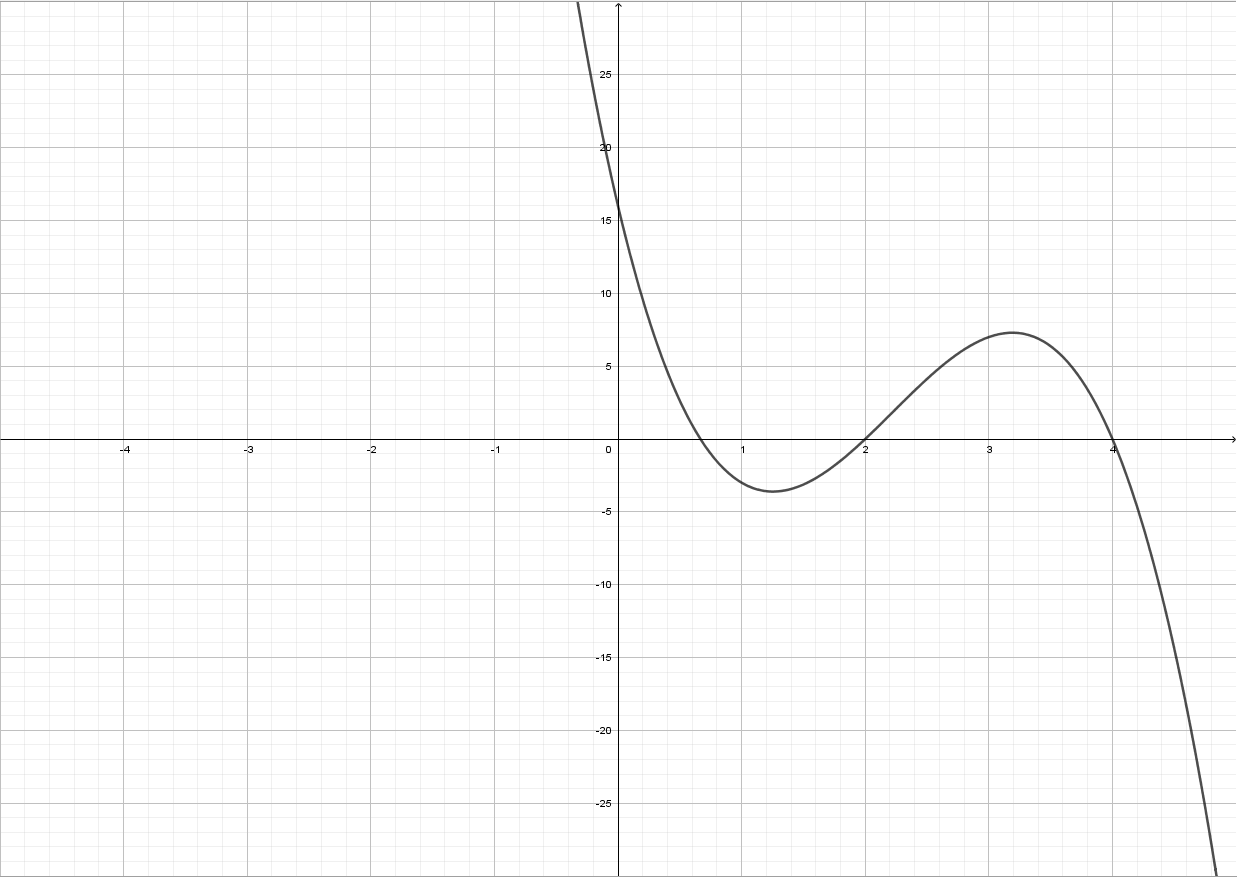
\includegraphics[width=3in]{3434b.png} \\
	Based on the graph, it is clear that one of the zeros will be between $\dfrac12$ and $1$, another will be $2$, and the third will be $4$. So we will test the following values of $x$: $\dfrac23$, $2$, and $4$.
	
	(c) \begin{tabular}{ccccc}
		$2/3$ & $-3$ & $20$ & $-36$ & $16$ \\
		& & $-2$ & $12$ & $-16$ \\
		& $-3$ & $18$ & $-24$ & $0$
	\end{tabular} \tabto{0.5\textwidth}
	$\polyhornerscheme[x = 2]{-3x^3 + 20x^2 - 36x + 16}$ \\
	$\polyhornerscheme[x = 4]{-3x^3 + 20x^2 - 36x + 16}$
	
	The Linear Factorization Theorem states that since $f$ is a cubic function, it has three zeros. Since we have found three zeros, we know that we have found all of the real zeros of $f$.
	
	% \vspace{}
	\vfill \newpage
	
	\begin{bex}{3.4.58}
		{
			
		}
	\end{bex} \vspace{-8pt}
	
	% My answer here
	We are told that $-4 + i$ is a zero of $g$. Since complex zeros occur in conjugate pairs, it follows that $-4 - i$ is a factor of $g$. Hence, $(x - (-4 + i))$ and $(x - (-4 - i))$ are factors of $g$, and so is their product. \begin{flalign*}
	\fp{x - (-4 + i)}\fp{x - (-4 - i)} &= (x + 4 - i)(x + 4 + i) & \\
	&= x^2 + 4x + ix + 4x + 16 + 4i - ix - 4i - i^2 & \\
	&= x^2 + 8x + 16 - i^2 & \\
	&= x^2 + 8x + 17
	\end{flalign*}
	So if we divide $x^3 + 9x^2 + 25x + 17$ by $x^2 + 8x + 17$, we will find our third zero.
	
	$\polylongdiv{x^3 + 9x^2 + 25x + 17}{x^2 + 8x + 17}$
	
	Therefore, the zeros of $g$ are: $x = -4 + i$, $x = -4 - i$, and $x = -1$
	
	% \vspace{}
	\vfill % \newpage
	
	\begin{bex}{3.4.74}
		{
			
		}
	\end{bex} \vspace{-8pt}
	
	% My answer here
	Factors of $-5$: $\pm 1$, $\pm, 5$ \\
	Factors of $2$: $\pm 1, \pm 2$
	
	Possible Rational Zeros: $\pm 1, \pm 5, \pm\dfrac12, \pm\dfrac52$
	
	There are only eight possible combinations; it should be quick to test until we find one then use factoring or the quadratic formula to find the other two (we know there will only be three since $f$ is a cubic function).
	
	$\polyhornerscheme[x = 1]{2x^3 - 5x^2 + 12x - 5}$ \tabto{0.5\textwidth} $\polyhornerscheme[x = -1]{2x^3 - 5x^2 + 12x - 5}$ \\
	$\polyhornerscheme[x = 2]{2x^3 - 5x^2 + 12x - 5}$ \tabto{0.5\textwidth} $\polyhornerscheme[x = -2]{2x^3 - 5x^2 + 12x - 5}$ \\
	\begin{tabular}{ccccc}
		$1/2$ & $2$ & $-5$ & $12$ & $-5$ \\
		& & $1$ & $-2$ & $5$ \\
		& $2$ & $-4$ & $10$ & $0$
	\end{tabular}
	\vfill \newpage
	
	So $2x^3 - 5x^2 + 12x - 5 = \fp{x - \dfrac12}\fp{2s^2 - 4s + 10} = 2\fp{s - \dfrac12}\fp{s^2 - 2s + 5}$. $s^2 - 2s + 5$ cannot be factored, so we can use the quadratic formula to find the other two values of $s$. \begin{flalign*}
	s^2 - 2s + 5 &= 0 & \\
	s &= \dfrac{2\pm\sqrt{(-2)^2 - 4(1)(5)}}{2(1)} & \\
	&= \dfrac{2\pm\sqrt{-16}}{2} & \\
	&= \dfrac{2\pm 4i}{2} & \\
	&= 1 \pm 2i
	\end{flalign*}
	So the three zeros of $f$ are $s = 1 + 2i$, $s = 1 - 2i$, and $s = \dfrac12$.
	
	
\end{document}